\documentclass[11pt,a4paper]{article}
\usepackage[margin=22mm,top=19mm,bottom=19mm]{geometry}
\usepackage{fontspec}\setmainfont{Cambria}\setsansfont{Calibri}\setmonofont{Consolas}[Scale=.9]
\usepackage{amsmath,amssymb,graphicx,booktabs,array,xcolor}
\setlength{\parindent}{0pt}\setlength{\parskip}{6pt}\setlength{\emergencystretch}{2em}
\renewcommand{\arraystretch}{1.18}\setlength{\tabcolsep}{5pt}
\newcommand{\heading}[2]{{\sffamily\small\color{blue!40!black}#1}\par{\sffamily\LARGE\bfseries#2}\par\vspace{3mm}}
\newcommand{\page}[2]{\newpage\heading{#1}{#2}}
\begin{document}
\heading{Proje kurgusu ve hesaplanabilir kapanış | 21 Eylül 2026}{Gereksinimden tamamlanmış projeye\\Sıfır açık karara ulaşan beş yöntem}
\textbf{Amaç.} Gereksinimin ilk yorumundan ara çalışmalara, tasarım kararlarına,
prototipe ve kabul edilmiş ürüne ilerleyen bir proje akışı kurmak.
Önceki rapordaki hücresel otomat resmine bu kez bir \emph{karar kaydı} eklenir.
Karar kaydı hangi konuların açık, hangilerinin kapalı olduğunu belirler;
resim bu akışın sembolik izini gösterir.

\begin{quote}\itshape
``Kapı mekanizması, ilkokul çağındaki bir çocuğun bile hiç zorlanmadan tek eliyle
açıp kapatabileceği bir tasarıma sahip olmalıdır.''
\end{quote}
Başlangıç, önceki rapordaki $011101000$ satırıdır. Dört siyah hücre dört açık
konuya bağlanır. Bunların sırasıyla yaş kapsamı, referans kullanıcı profili,
kuvvet sınırı ve açma-kapama kapsamı olduğu açıkça kaydedilir.

\section*{Bu raporda ``0 belirsizlik'' ne demektir?}
Proje sonunda tanımlı kapsam için tek bir tasarım paketi seçilmiş, dört açık
konu kapatılmış ve dört kabul kaydı doğrulanmış olmalıdır:
\[
|\Omega_T|=1,\quad U_T=0,\quad O_T=0,\quad V_T=4.
\]
$\Omega_T$ açık tasarım paketleri kümesi, $U_T$ proje karar entropisi,
$O_T$ açık konu sayısı, $V_T$ doğrulanmış kabul kaydı sayısıdır.
Bu koşul, projenin tanımlı karar kapsamındaki kapanışıdır; gelecekte hiç arıza,
ölçüm hatası veya yeni gereksinim olmayacağı anlamına gelmez.

\textbf{Üç katman.} (1) Gereksinim ve alternatifler; (2) ara çalışmalar,
bağlayıcı kararlar ve kabul kayıtları; (3) bunların görsel izi ve sayısal ölçümleri.
Kural 0 ile resmi silmek yalnız üçüncü katmanı değiştirir. Projeyi tamamlamak
için ilk iki katmanın da kapanması gerekir.

\textbf{Deneyin statüsü.} Bu belgede anlatılan beş akış birer başarı senaryosu
simülasyonudur. Prototipler ve kabul sonuçları gerçek ölçüm değildir.
Verilen sayısal sınırlar örnek tasarım girdileridir; çocuklara uygunluk veya
bir standarda uyum iddiası taşımaz. Başarısız test durumunda kapanış verilmez.

\page{Ortak örnek proje}{1\quad Dört açık konu, 16 tasarım paketi}
Her konu için yalnız iki seçenek tanımlıyoruz. Bu sınırlı alternatif uzayı
hesabı izlenebilir kılar; bütün gerçek tasarım olanaklarını kapsamaz.
\begin{center}\small\begin{tabular}{c p{40mm} p{43mm} p{43mm}}\toprule
Konu & Açık soru & 0 seçeneği & 1 seçeneği\\\midrule
A & Kullanıcı kapsamı & 8--12 yaş kapsamı & 6--12 yaş kapsamı\\
B & Referans test profili & P0: küçük el fikstürü & P1: orta el fikstürü\\
C & Tepe işletme kuvveti & 15 N tasarım hedefi & 10 N tasarım hedefi\\
D & İşlev kapsamı & Yalnız mandal çözme & Tam açma ve kapama\\\bottomrule
\end{tabular}\end{center}
P0 ve P1, proje içinde ayrıca boyutlandırılıp tanımlanacak iki test düzeneği
profilidir. Bunları gerçek çocuk davranışına eşitlemiyoruz. Mekanizma geometrisi,
kol uzunluğu ve sürtünme azaltma çalışmaları C hedefini sağlamak için yapılır.
Bu rapor dört konunun kapanışını izler; ayrıntılı mekanik boyutlandırma yapmaz.

\textbf{Başlangıç.} $\Omega_0=\{0,1\}^4$ ve her paket için $p_0=1/16$.
Bu eş olasılıklılık bir başlangıç modellemesi varsayımıdır.
\[
U_0=-\sum_{a\in\Omega_0}\frac1{16}\log_2\frac1{16}=4\ \text{bit}.
\]
Örnek hedef paket $a^*=1011$'dir: A=1, B=0, C=1, D=1.
Paketin ikili 0'ları ``çözülmemiş'' anlamına gelmez; alternatif kimliğidir.
Resimdeki 0 ise açık konu izi bulunmayan hücredir. İki kod birbirinden ayrıdır.

\textbf{Kapanışta yazılacak gereksinim.}
\begin{quote}
Proje, 6--12 yaş kullanıcı kapsamını esas alacaktır. P0 referans fikstüründe,
tanımlı test düzeneğinde ölçülen tepe işletme kuvveti 10 N'yi aşmadan,
tek elle mandalın çözülmesi, kapının $0^\circ$'den $90^\circ$'ye açılması
ve yeniden kapatılması tamamlanacaktır.
\end{quote}
Bu cümledeki P0 çizimi, test hızı ve koşulları kabul planında sabitlenmeden
gerçek proje kapanamaz. Simülasyonda bunların tamamlanmış olduğu varsayılır.

\textbf{Dört kabul kaydı.} K1: kullanıcı kapsamı onaylıdır; K2: P0 çizimi ve
test prosedürü onaylıdır; K3: seçilen kuvvet hedefi prototipte sağlanmıştır;
K4: tam açma-kapama işlevi bütünleşik testte sağlanmıştır. Bu rapor gerçek
test sonucu üretmez; başarılı kapanış yolunda K1--K4 için ``geçti'' girdisi kullanır.

\page{Hesaplama çerçevesi}{2\quad Proje belirsizliği ve resim entropisi}
\textbf{Proje karar entropisi.} Olasılığı pozitif paketler üzerinden:
\[
U_t=-\sum_{a\in\Omega_t}p_t(a)\log_2p_t(a).
\]
Eş olasılıklı $M_t$ paket varsa $U_t=\log_2 M_t$ olur. $M_t=1$ için $U_t=0$.
Olasılık taşıyan paketler bir konuda aynı seçeneği vermiyorsa o konu açıktır:
\[
O_t=\sum_{j=1}^4\mathbf1\{\exists a,b:\ p_t(a)>0,\ p_t(b)>0,\ a_j\ne b_j\}.
\]
Dört konunun bağımlı olduğu durumlarda $O_t$ ile $U_t$ aynı sayı değildir.
Örneğin iki paket, dört konunun tamamında farklıysa $U=1$ bit, $O=4$ olabilir.

\textbf{Güncel resim.} Adım $t$'de $N_t=9+2t$ hücre vardır. Siyah sayısı
$b_t$ ise $q_t=b_t/N_t$ ve
\[
H_{1,t}=-q_t\log_2q_t-(1-q_t)\log_2(1-q_t).
\]
İkili desen entropisi $H_{2,t}$, $00,01,10,11$ çiftlerinin $N_t-1$ adet
örtüşen konumdaki frekanslarından hesaplanır; CSV dosyalarında verilmiştir.

\textbf{Geçmiş resim.} $0,\ldots,t$ satırlarının geçerli hücreleri birleştirilir:
\[
A_t=(t+1)(9+t),\quad B_t=\sum_{s=0}^t b_s,\qquad
H_{\mathrm{geçmiş},t}=h_2(B_t/A_t).
\]
Burada $h_2$ ikili entropi fonksiyonudur. Son satır beyaz olsa bile önceki
siyah hücreler durduğu için geçmişin entropisi genellikle sıfır olmaz.
Bu, kapanışın başarısız olduğu anlamına gelmez; tamamlanan projenin geçmişidir.

\textbf{Yanlış sıfır örneği.} Tam siyah ve tam beyaz iki satırın da renk
entropisi sıfırdır. Tam siyah satırı ``bütün konular çözüldü'' diye okuyamayız.
Bu yüzden kapanış kararı $H_1=0$ testinden değil, $U=0$, $O=0$ ve kabul
kayıtlarından verilir. Resim bu kararı izler.

\textbf{Boş küme başarısızlıktır.} $\Omega_t=\varnothing$ olduğunda olasılıklar
normalize edilemez. Bunu $U=0$ olarak kaydetmiyoruz: gereksinimler çelişkili
veya bütün adaylar başarısızdır; karar geri alınır ya da tasarım genişletilir.

\page{Kararlardan resme}{3\quad Ara çalışma ve karar operatörü}
\textbf{Ara çalışma.} İlk olarak bir hücresel otomat kuralı uygulanır:
\[
z_{t+1,i}=F_{r_t}(x_{t,i-1},x_{t,i},x_{t,i+1}).
\]
Kural 90/150 farklı ilişkileri yaymayı, 30/110 seçenek etkileşimlerini,
232 yerel birleştirmeyi, 184 aktarımı, 204 mevcut tasarımı korumayı temsil
etmek üzere seçilmiş görsel benzetmelerdir. Bunların gerçek tasarımcı
davranışına eşdeğerliği doğrulanmış değildir.

\textbf{Konu etiketleri.} Başlangıçtaki dört siyah hücre sırayla
$\{A\},\{B\},\{C\},\{D\}$ etiketi taşır; beyazların etiketi boştur.
Yeni hücre, sol/merkez/sağ etiketlerinin birleşimini devralır. Bu,
kesin nedensel analiz değil, muhafazakâr bir yerel izleme yöntemidir.

\textbf{Karar kapısı.} Çalışma çıktısı aday kümesini veya olasılıkları
günceller. Açık konular kümesi $\mathcal O_{t+1}$ bulunur. Sonra:
\[
\widetilde L_{t+1,i}=(L_{t,i-1}\cup L_{t,i}\cup L_{t,i+1})\cap\mathcal O_{t+1},
\]
\[
x_{t+1,i}=z_{t+1,i}\,\mathbf1\{\widetilde L_{t+1,i}\ne\varnothing\}.
\]
Çıktı beyazsa etiketi boşaltılır. Böylece kapanmış konuların tek başına
ürettiği izler silinir; açık konuya bağlı izler kalabilir. Bir hücrenin
beyazlaşması kayıtlı konuyu kendi başına kapatmaz.

\textbf{Son adım neden sıfır?} Son karar ve kabul sonrasında
$\mathcal O_T=\varnothing$ ise bütün etiket kesişimleri boştur. Bu yüzden
$x_{T,i}=0$ ve $H_{1,T}=H_{2,T}=0$ olur. Bu sonuç hücresel otomatın
kendiliğinden yakınsamasından değil, açıkça tanımlanmış karar operatöründen gelir.

\textbf{Sıra.} Her adımda önce geçici resim, sonra karar güncellemesi,
sonra etiket süzme ve entropi hesabı yapılır. Grafiklerdeki turuncu yatay
çizgiler $t=6,12,18,24$ çalışma/karar noktalarıdır. Adımlar gerçek takvim
günü değildir. Dört evrede kullanılacak kural dizileri sonraki sayfalardadır.

\textbf{Başarısız dal.} Kabul kaydı geçmezse proje tamamlandı olarak işaretlenmez.
İlgili konu yeniden açılır, aday kümesi güncellenir ve yeni iterasyon başlatılır.
Buradaki MATLAB örneği yalnız başarılı dalı çalıştırır; başarısızlık halinde
otomatik düzeltme yaptığı iddia edilmez.

\page{Yöntem 1/5 | Proje akışı}{4\quad Sıralı karar kapıları}
\textbf{Ara çalışma kuralları.} $t=1\!:\!6,\ 7\!:\!12,\ 13\!:\!18,\ 19\!:\!24$ evrelerinde sırasıyla 90, 150, 232, 204 uygulanır. Karar operatörü bu yerel kurallardan ayrıdır.
\begin{center}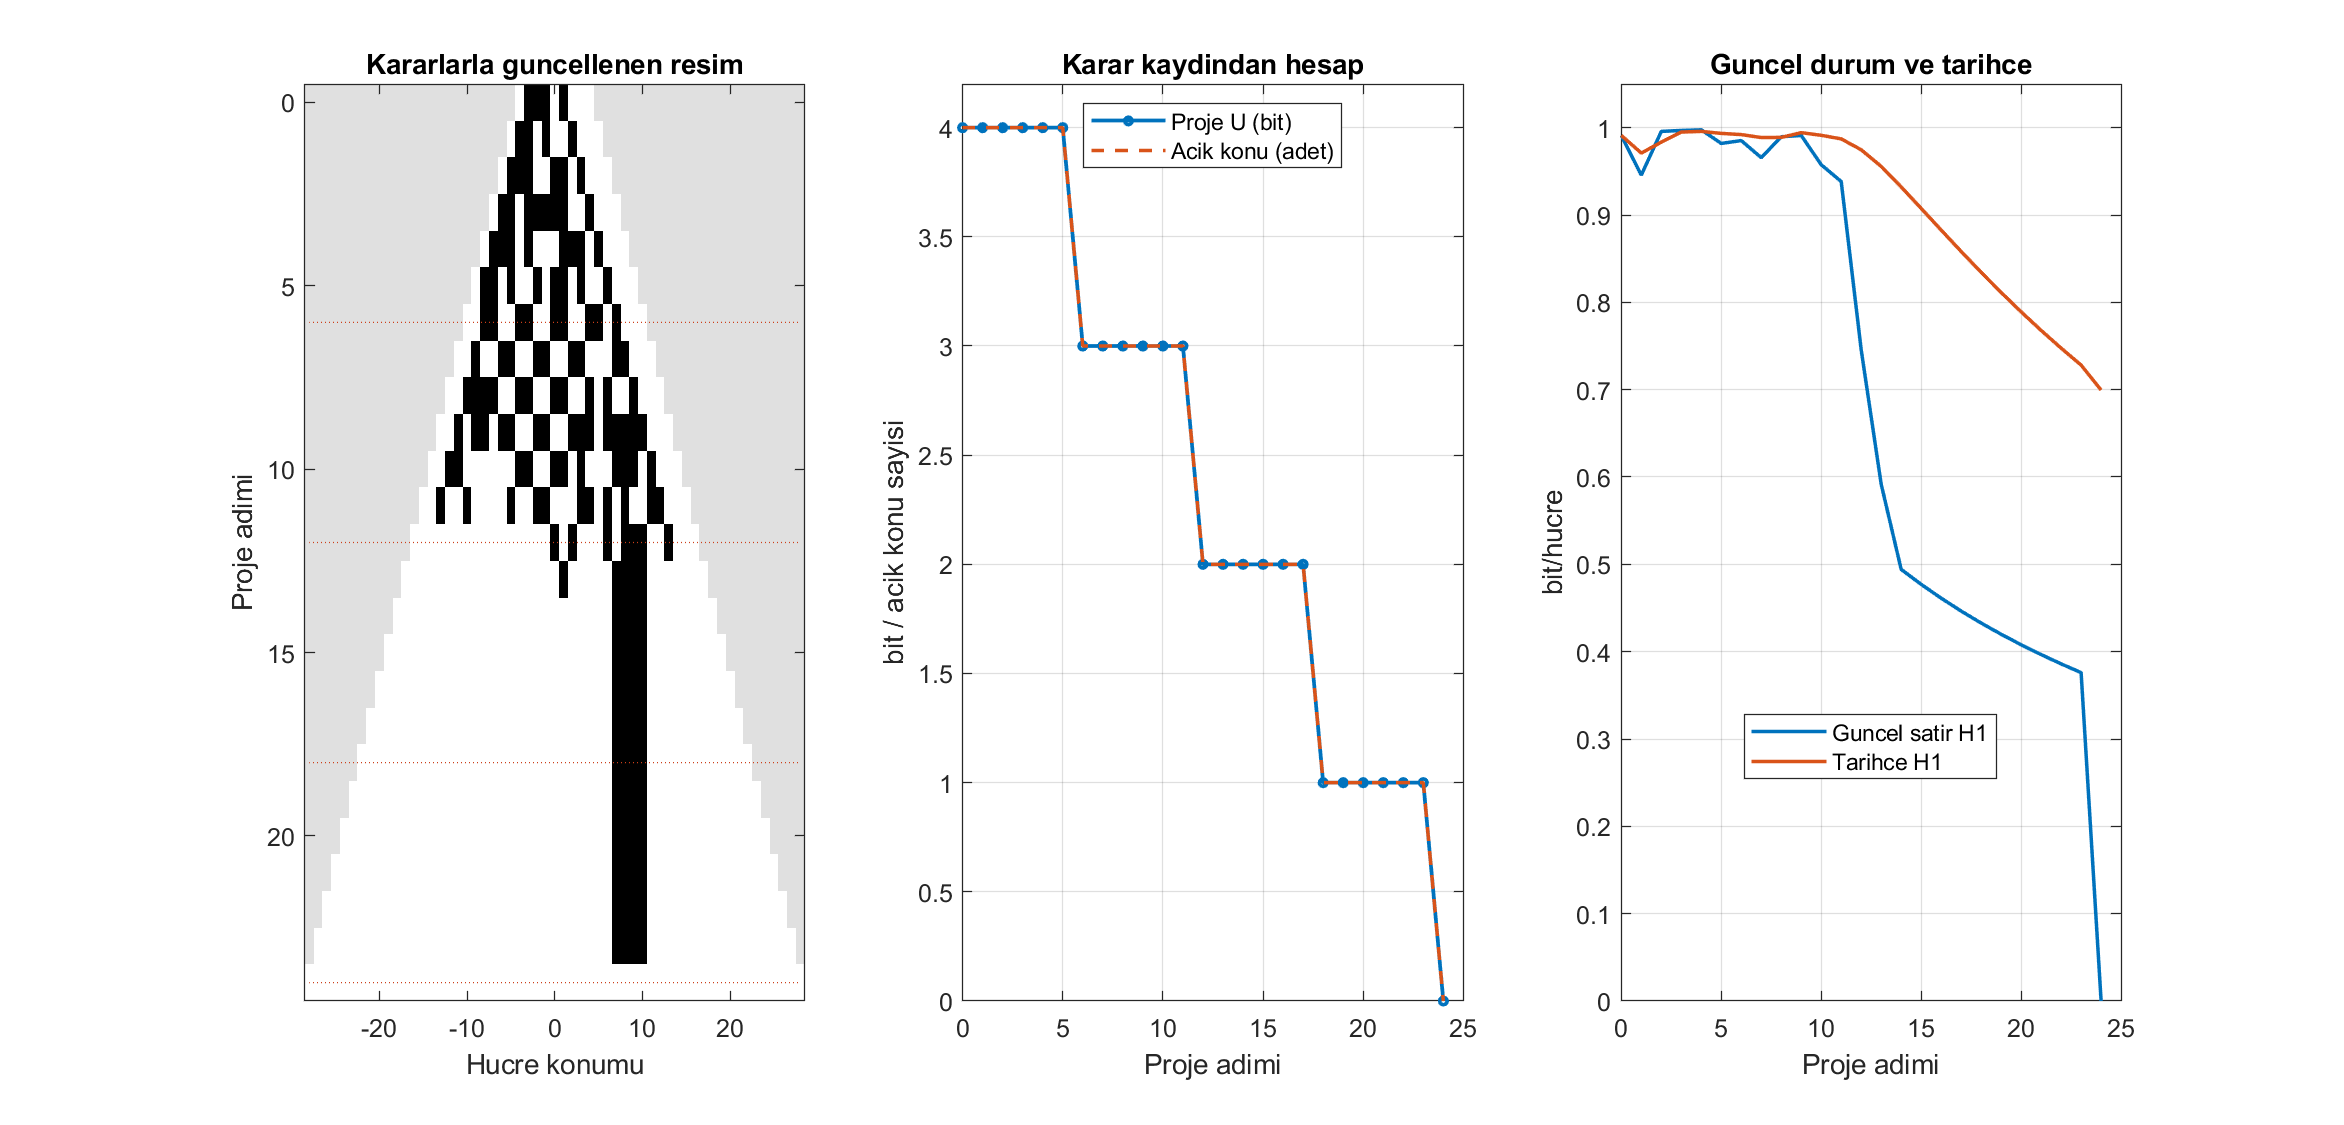
\includegraphics[width=\linewidth]{assets/method_1.png}\end{center}
\begin{center}\small\begin{tabular}{r p{46mm} p{95mm}}\toprule $t$ & Ara çalışma & Karar veya çıktı\\\midrule
6 & Kullanıcı kapsamı çalışması & A=1; 6–12 yaş kapsamı onaylanır. \\
12 & Referans profil incelemesi & B=0; P0 test düzeneği seçilir. \\
18 & Kuvvet bütçesi ve mekanizma hesabı & C=1; 10 N hedefi ve buna göre kol tasarımı. \\
24 & Tam prototip ve kabul testi & D=1; tam açma-kapama, dört kayıt doğrulanır. \\
\bottomrule\end{tabular}\end{center}
\textbf{Yorum.} Her kapı tek bir konuyu kapatır. Eş olasılıklı aday sayısı 16, 8, 4, 2 ve 1 olur; proje entropisi her kapıda bir bit azalır. Kararlar izlenebilir fakat sonraki iş önceki kapıyı bekler. Geç bir test önceki kararı geçersiz kılarsa ilgili kapı yeniden açılır.

\textbf{Sonuç.} Başarılı kabul girdisi altında tek paket 1011 kalır; $U_{24}=0$, $O_{24}=0$, $V_{24}=4$ ve son satır tamamen beyazdır. Geçmiş satırlar korunur.

\page{Yöntem 1/5 | Hesap ve izlenebilirlik}{Sıralı karar kapıları: sayısal sonuçlar}
Karar noktalarındaki paket sayıları 16, 8, 4, 2, 1; bunların $\log_2$ değerleri sırasıyla 4,0000, 3,0000, 2,0000, 1,0000, 0,0000 bittir.
\begin{center}\small\begin{tabular}{rrrrrrr}\toprule $t$ & Aday & Açık konu & Proje $U$ & Satır $H_1$ & Geçmiş $H_1$ & Kabul\\\midrule
0 & 16 & 4 & 4,0000 & 0,9911 & 0,9911 & 0/4 \\
1 & 16 & 4 & 4,0000 & 0,9457 & 0,9710 & 0/4 \\
2 & 16 & 4 & 4,0000 & 0,9957 & 0,9834 & 0/4 \\
3 & 16 & 4 & 4,0000 & 0,9968 & 0,9950 & 0/4 \\
4 & 16 & 4 & 4,0000 & 0,9975 & 0,9957 & 0/4 \\
5 & 16 & 4 & 4,0000 & 0,9819 & 0,9934 & 0/4 \\
6 & 8 & 3 & 3,0000 & 0,9852 & 0,9921 & 0/4 \\
7 & 8 & 3 & 3,0000 & 0,9656 & 0,9887 & 0/4 \\
8 & 8 & 3 & 3,0000 & 0,9896 & 0,9888 & 0/4 \\
9 & 8 & 3 & 3,0000 & 0,9911 & 0,9943 & 0/4 \\
10 & 8 & 3 & 3,0000 & 0,9576 & 0,9912 & 0/4 \\
11 & 8 & 3 & 3,0000 & 0,9383 & 0,9871 & 0/4 \\
12 & 4 & 2 & 2,0000 & 0,7455 & 0,9747 & 0/4 \\
13 & 4 & 2 & 2,0000 & 0,5917 & 0,9556 & 0/4 \\
14 & 4 & 2 & 2,0000 & 0,4942 & 0,9321 & 0/4 \\
15 & 4 & 2 & 2,0000 & 0,4771 & 0,9075 & 0/4 \\
16 & 4 & 2 & 2,0000 & 0,4612 & 0,8827 & 0/4 \\
17 & 4 & 2 & 2,0000 & 0,4465 & 0,8582 & 0/4 \\
18 & 2 & 1 & 1,0000 & 0,4328 & 0,8344 & 0/4 \\
19 & 2 & 1 & 1,0000 & 0,4199 & 0,8113 & 0/4 \\
20 & 2 & 1 & 1,0000 & 0,4079 & 0,7891 & 0/4 \\
21 & 2 & 1 & 1,0000 & 0,3966 & 0,7678 & 0/4 \\
22 & 2 & 1 & 1,0000 & 0,3860 & 0,7475 & 0/4 \\
23 & 2 & 1 & 1,0000 & 0,3760 & 0,7281 & 0/4 \\
24 & 1 & 0 & 0,0000 & 0,0000 & 0,6996 & 4/4 \\
\bottomrule\end{tabular}\end{center}
\textbf{Hesap ayrımı.} Proje $U$ değeri paket olasılıklarından; satır ve geçmiş değerleri hücre frekanslarından hesaplanır. Hepsi bit tabanını kullanır, fakat aynı rastgele değişkenin entropisi değildir. Son satırın genişliği 57, geçmişin alanı 825 hücredir.

\page{Yöntem 2/5 | Proje akışı}{5\quad Paralel alt çalışmalar}
\textbf{Ara çalışma kuralları.} $t=1\!:\!6,\ 7\!:\!12,\ 13\!:\!18,\ 19\!:\!24$ evrelerinde sırasıyla 30, 90, 184, 232 uygulanır. Karar operatörü bu yerel kurallardan ayrıdır.
\begin{center}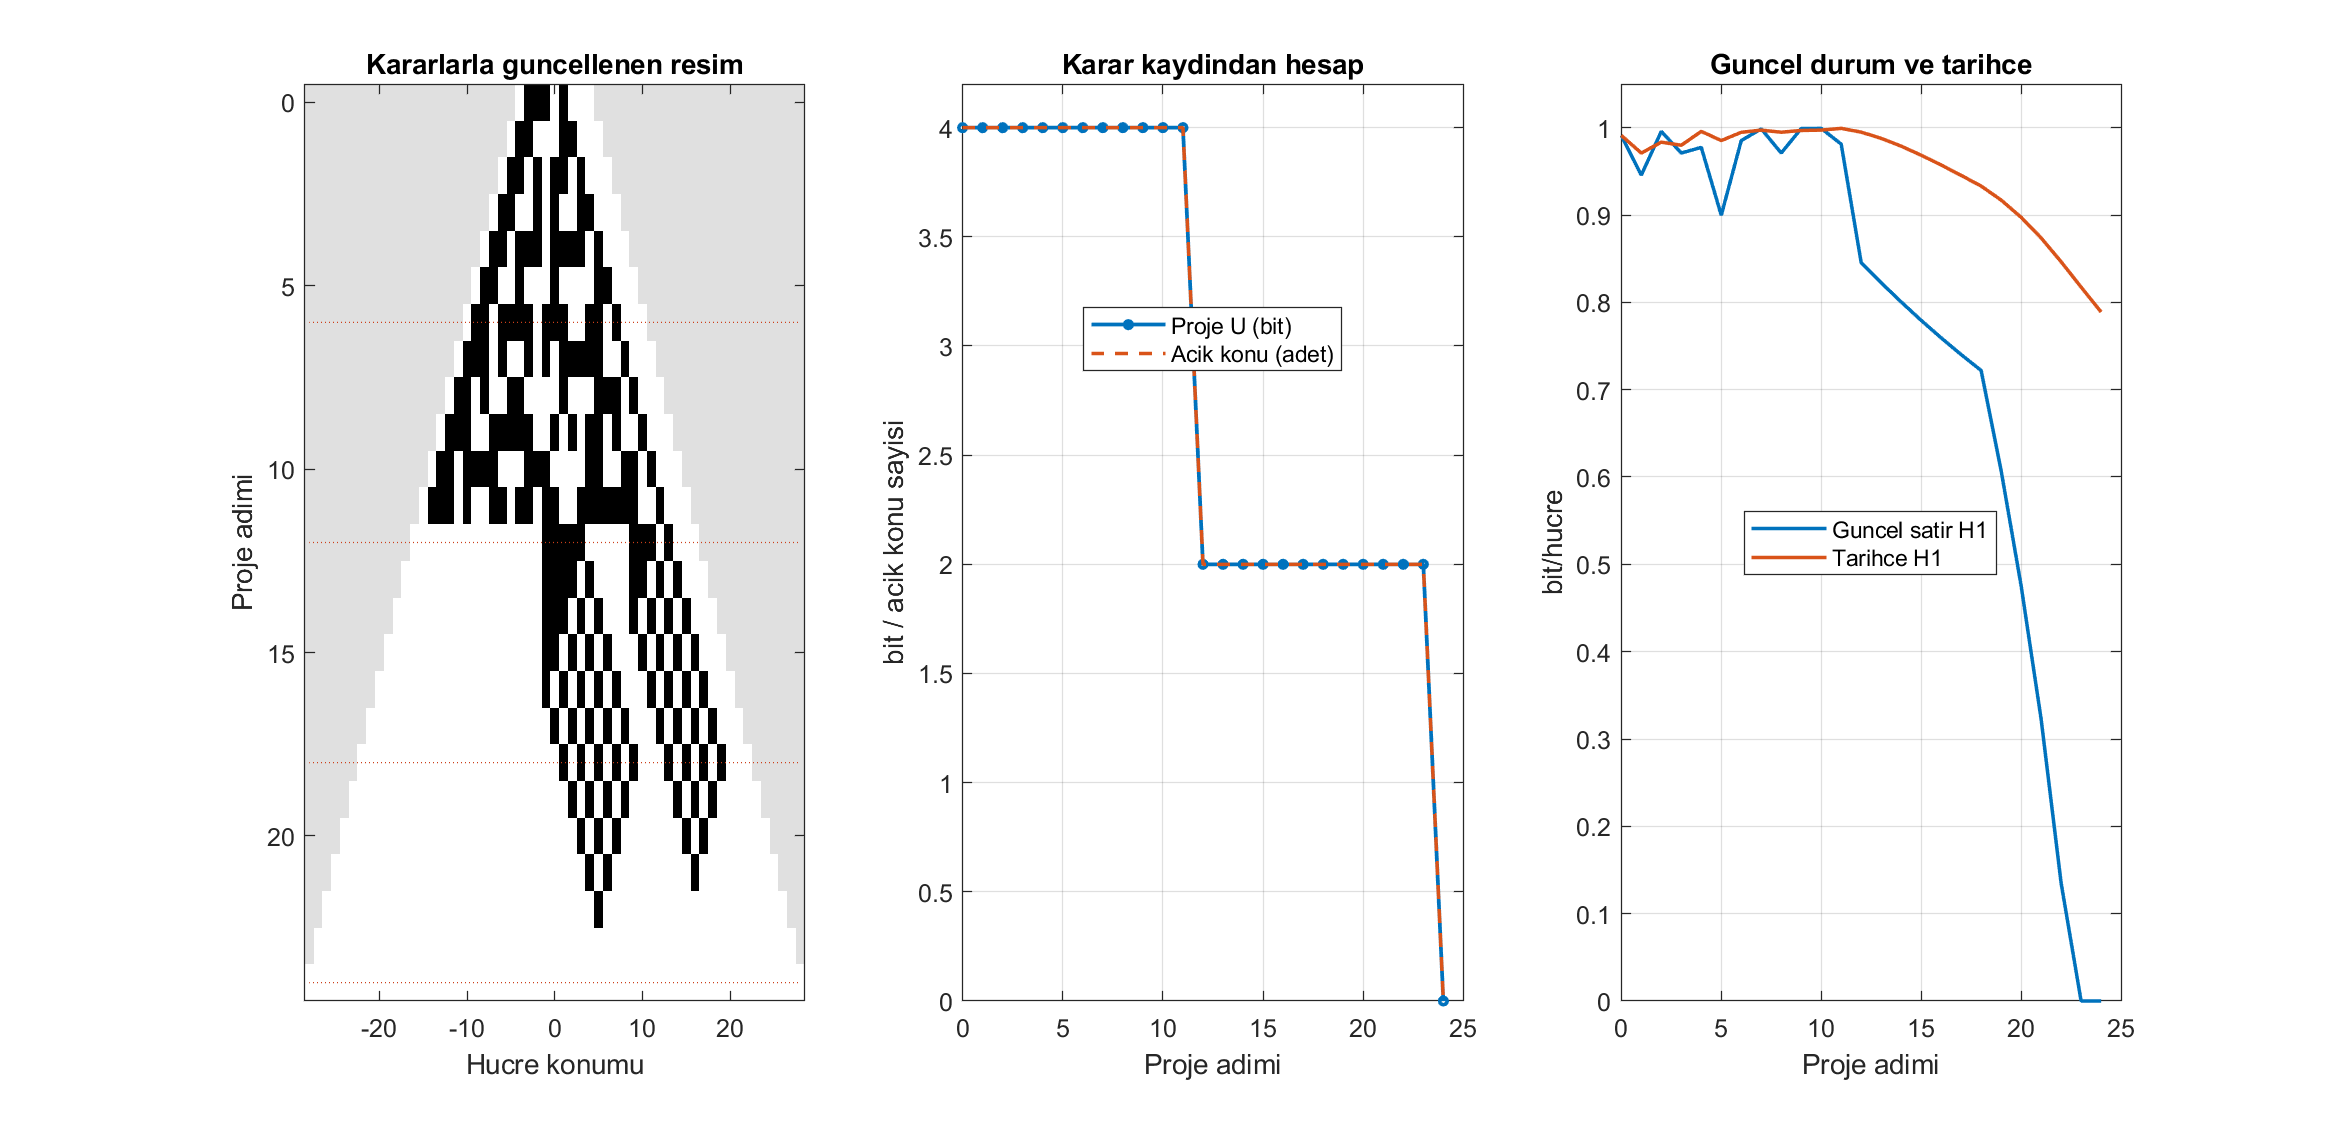
\includegraphics[width=\linewidth]{assets/method_2.png}\end{center}
\begin{center}\small\begin{tabular}{r p{46mm} p{95mm}}\toprule $t$ & Ara çalışma & Karar veya çıktı\\\midrule
6 & İki iş paketi eşzamanlı başlar & Kapsam/profil ekibi ile mekanizma/test ekibi çalışır. \\
12 & İlk paket teslimi & A=1 ve B=0 birlikte sabitlenir. \\
18 & Mekanizma prototipi ve arayüz kontrolü & C ve D henüz açıktır; kabul kararı beklenir. \\
24 & Birleştirme ve bütün sistem testi & C=1, D=1; tüm kayıtlar doğrulanır. \\
\bottomrule\end{tabular}\end{center}
\textbf{Yorum.} İlk iki konu ile son iki konu ayrı iş paketlerinde çözülür. Bu örnekte entropi iki büyük adımda 4, 2 ve 0 bite iner. Paralellik takvim kazancı sağlayabilir; fakat bunu bu adım sayılarıyla ölçmüş değiliz. Son kapıda alt sistemlerin tek başına çalışması yetmez, birlikte çalışmaları da doğrulanır.

\textbf{Sonuç.} Başarılı kabul girdisi altında tek paket 1011 kalır; $U_{24}=0$, $O_{24}=0$, $V_{24}=4$ ve son satır tamamen beyazdır. Geçmiş satırlar korunur.

\page{Yöntem 2/5 | Hesap ve izlenebilirlik}{Paralel alt çalışmalar: sayısal sonuçlar}
Karar noktalarındaki paket sayıları 16, 16, 4, 4, 1; bunların $\log_2$ değerleri sırasıyla 4,0000, 4,0000, 2,0000, 2,0000, 0,0000 bittir.
\begin{center}\small\begin{tabular}{rrrrrrr}\toprule $t$ & Aday & Açık konu & Proje $U$ & Satır $H_1$ & Geçmiş $H_1$ & Kabul\\\midrule
0 & 16 & 4 & 4,0000 & 0,9911 & 0,9911 & 0/4 \\
1 & 16 & 4 & 4,0000 & 0,9457 & 0,9710 & 0/4 \\
2 & 16 & 4 & 4,0000 & 0,9957 & 0,9834 & 0/4 \\
3 & 16 & 4 & 4,0000 & 0,9710 & 0,9799 & 0/4 \\
4 & 16 & 4 & 4,0000 & 0,9774 & 0,9957 & 0/4 \\
5 & 16 & 4 & 4,0000 & 0,8997 & 0,9852 & 0/4 \\
6 & 16 & 4 & 4,0000 & 0,9852 & 0,9947 & 0/4 \\
7 & 16 & 4 & 4,0000 & 0,9986 & 0,9972 & 0/4 \\
8 & 16 & 4 & 4,0000 & 0,9710 & 0,9948 & 0/4 \\
9 & 16 & 4 & 4,0000 & 0,9990 & 0,9968 & 0/4 \\
10 & 16 & 4 & 4,0000 & 0,9991 & 0,9972 & 0/4 \\
11 & 16 & 4 & 4,0000 & 0,9812 & 0,9992 & 0/4 \\
12 & 4 & 2 & 2,0000 & 0,8454 & 0,9949 & 0/4 \\
13 & 4 & 2 & 2,0000 & 0,8224 & 0,9878 & 0/4 \\
14 & 4 & 2 & 2,0000 & 0,8004 & 0,9788 & 0/4 \\
15 & 4 & 2 & 2,0000 & 0,7793 & 0,9685 & 0/4 \\
16 & 4 & 2 & 2,0000 & 0,7593 & 0,9572 & 0/4 \\
17 & 4 & 2 & 2,0000 & 0,7401 & 0,9453 & 0/4 \\
18 & 4 & 2 & 2,0000 & 0,7219 & 0,9331 & 0/4 \\
19 & 4 & 2 & 2,0000 & 0,6072 & 0,9171 & 0/4 \\
20 & 4 & 2 & 2,0000 & 0,4754 & 0,8973 & 0/4 \\
21 & 4 & 2 & 2,0000 & 0,3228 & 0,8738 & 0/4 \\
22 & 4 & 2 & 2,0000 & 0,1350 & 0,8464 & 0/4 \\
23 & 4 & 2 & 2,0000 & 0,0000 & 0,8174 & 0/4 \\
24 & 1 & 0 & 0,0000 & 0,0000 & 0,7889 & 4/4 \\
\bottomrule\end{tabular}\end{center}
\textbf{Hesap ayrımı.} Proje $U$ değeri paket olasılıklarından; satır ve geçmiş değerleri hücre frekanslarından hesaplanır. Hepsi bit tabanını kullanır, fakat aynı rastgele değişkenin entropisi değildir. Son satırın genişliği 57, geçmişin alanı 825 hücredir.

\page{Yöntem 3/5 | Proje akışı}{6\quad Kısıtlarla seçenek daraltma}
\textbf{Ara çalışma kuralları.} $t=1\!:\!6,\ 7\!:\!12,\ 13\!:\!18,\ 19\!:\!24$ evrelerinde sırasıyla 150, 232, 204, 204 uygulanır. Karar operatörü bu yerel kurallardan ayrıdır.
\begin{center}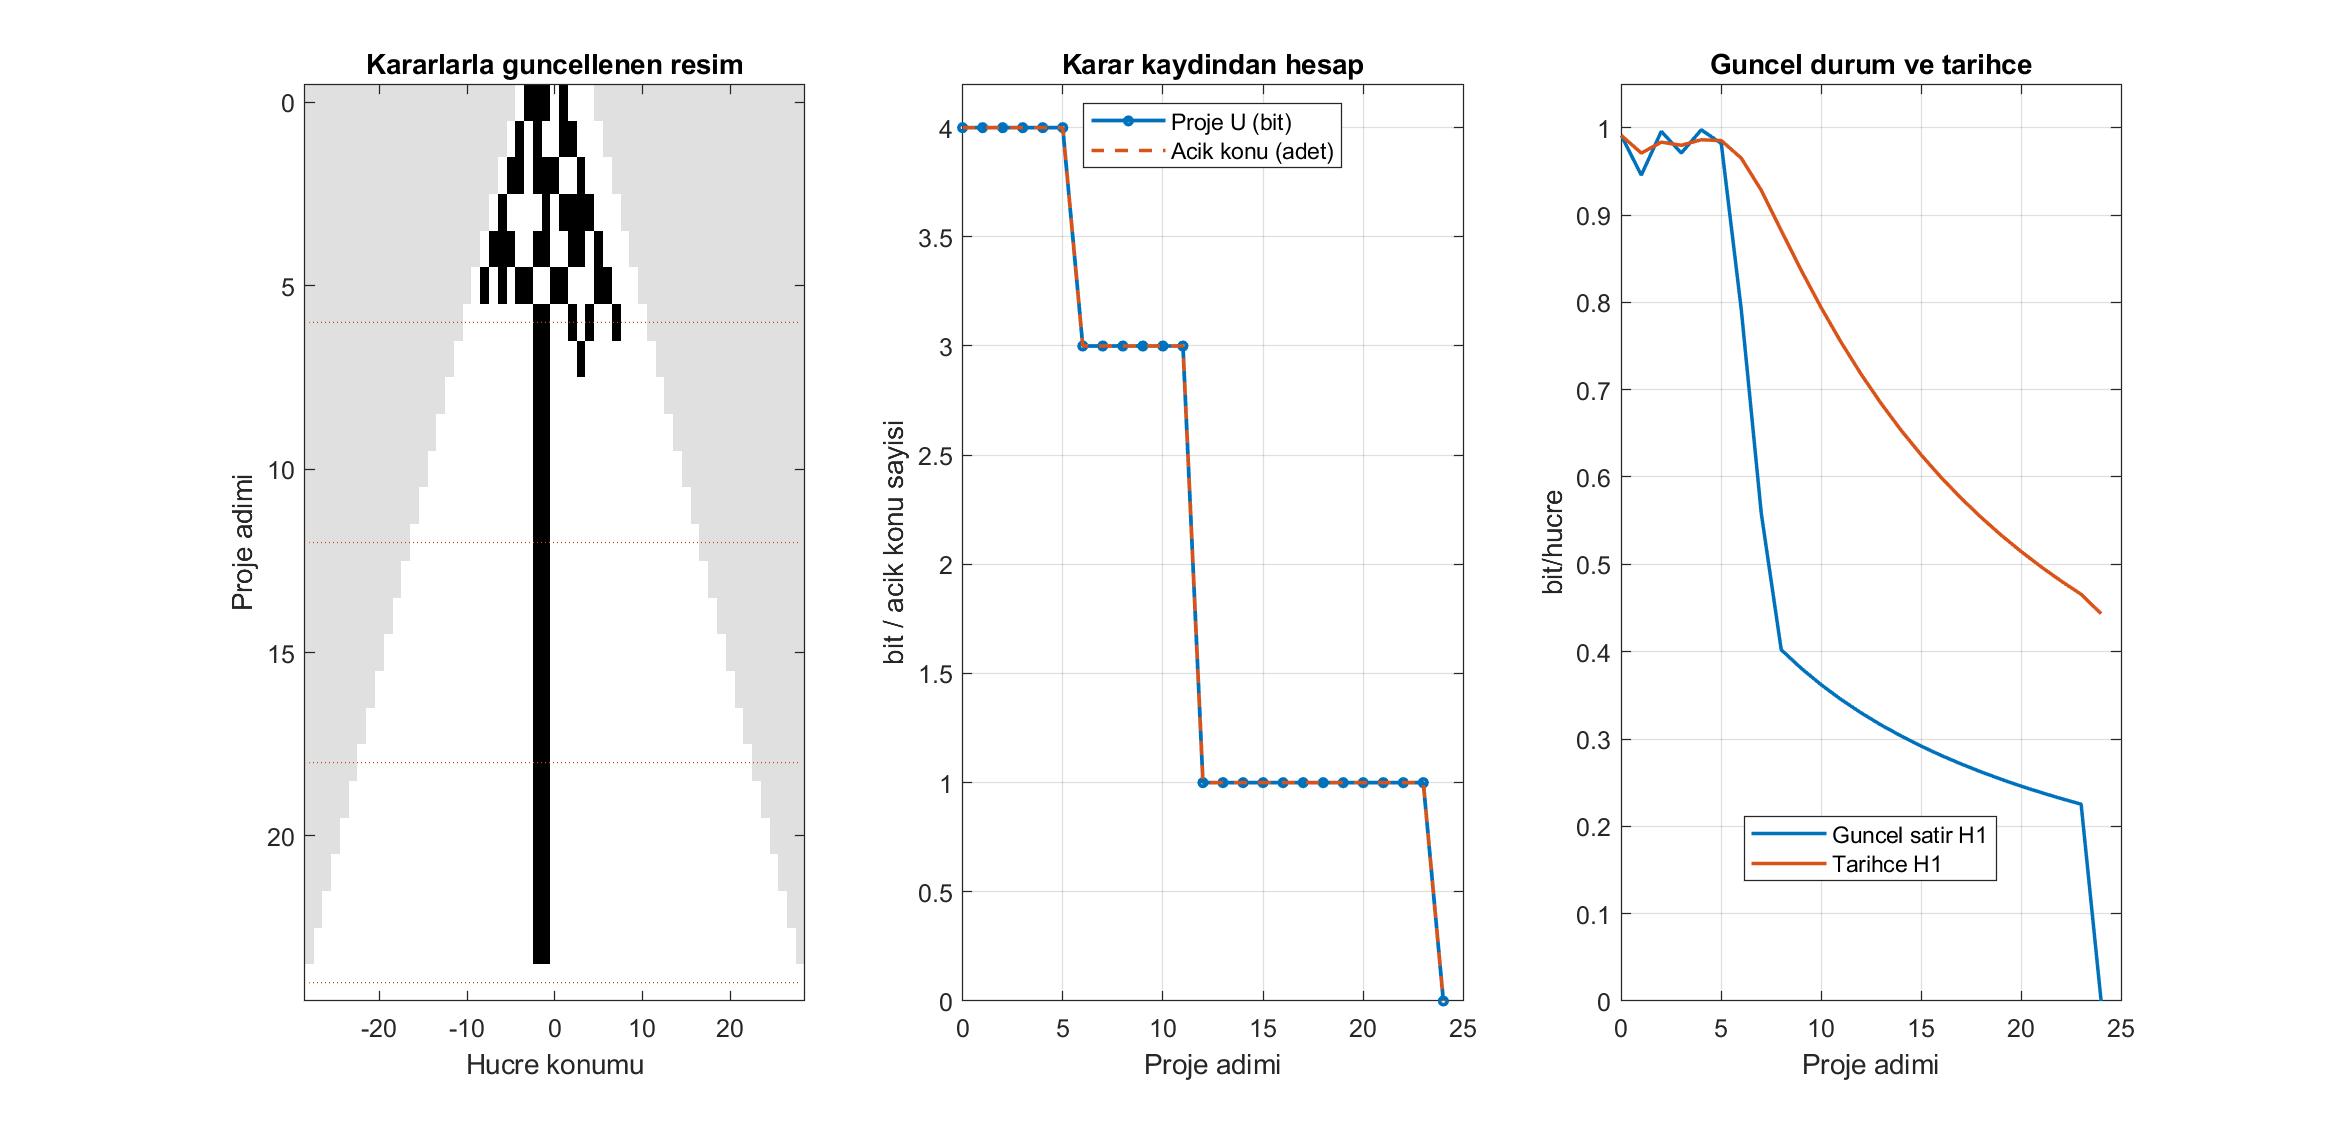
\includegraphics[width=\linewidth]{assets/method_3.png}\end{center}
\begin{center}\small\begin{tabular}{r p{46mm} p{95mm}}\toprule $t$ & Ara çalışma & Karar veya çıktı\\\midrule
6 & Kapsam kararı & A=1 seçilir. \\
12 & Tasarım bağlantı kuralları kabulü & B=1-A ve C=A; B=0 ve C=1 çıkar. \\
18 & Bağlantıların prototipte kontrolü & Yeni eleme yok; doğrulama hazırlığı. \\
24 & Fonksiyon kapsamı ve kabul & D=1; kısıtlar ve ürün birlikte doğrulanır. \\
\bottomrule\end{tabular}\end{center}
\textbf{Yorum.} Bir karar, kabul edilmiş bağlantılar aracılığıyla başka kararları da belirler. Buradaki B=1-A ve C=A bağıntıları fizik yasası veya yaşa ilişkin deneysel sonuç değildir; yalnız bu örnek proje için seçilen paketleme politikasıdır. Çelişki varsa aday kümesi boşalır; bu durum başarı değil, yeniden tasarım gerektirir.

\textbf{Sonuç.} Başarılı kabul girdisi altında tek paket 1011 kalır; $U_{24}=0$, $O_{24}=0$, $V_{24}=4$ ve son satır tamamen beyazdır. Geçmiş satırlar korunur.

\page{Yöntem 3/5 | Hesap ve izlenebilirlik}{Kısıtlarla seçenek daraltma: sayısal sonuçlar}
$t=6$ için A=1 olduğundan sekiz paket kalır: $U=\log_2 8=3$. $t=12$ bağlantıları B=0 ve C=1 yapar; yalnız D değişebilir: $U=\log_2 2=1$. $t=24$ için D=1 ve kabul, $U=0$ verir.
\begin{center}\small\begin{tabular}{rrrrrrr}\toprule $t$ & Aday & Açık konu & Proje $U$ & Satır $H_1$ & Geçmiş $H_1$ & Kabul\\\midrule
0 & 16 & 4 & 4,0000 & 0,9911 & 0,9911 & 0/4 \\
1 & 16 & 4 & 4,0000 & 0,9457 & 0,9710 & 0/4 \\
2 & 16 & 4 & 4,0000 & 0,9957 & 0,9834 & 0/4 \\
3 & 16 & 4 & 4,0000 & 0,9710 & 0,9799 & 0/4 \\
4 & 16 & 4 & 4,0000 & 0,9975 & 0,9861 & 0/4 \\
5 & 16 & 4 & 4,0000 & 0,9819 & 0,9852 & 0/4 \\
6 & 8 & 3 & 3,0000 & 0,7919 & 0,9651 & 0/4 \\
7 & 8 & 3 & 3,0000 & 0,5586 & 0,9284 & 0/4 \\
8 & 8 & 3 & 3,0000 & 0,4022 & 0,8821 & 0/4 \\
9 & 8 & 3 & 3,0000 & 0,3809 & 0,8366 & 0/4 \\
10 & 8 & 3 & 3,0000 & 0,3621 & 0,7938 & 0/4 \\
11 & 8 & 3 & 3,0000 & 0,3451 & 0,7540 & 0/4 \\
12 & 2 & 1 & 1,0000 & 0,3298 & 0,7175 & 0/4 \\
13 & 2 & 1 & 1,0000 & 0,3160 & 0,6840 & 0/4 \\
14 & 2 & 1 & 1,0000 & 0,3034 & 0,6534 & 0/4 \\
15 & 2 & 1 & 1,0000 & 0,2918 & 0,6253 & 0/4 \\
16 & 2 & 1 & 1,0000 & 0,2812 & 0,5994 & 0/4 \\
17 & 2 & 1 & 1,0000 & 0,2714 & 0,5757 & 0/4 \\
18 & 2 & 1 & 1,0000 & 0,2623 & 0,5537 & 0/4 \\
19 & 2 & 1 & 1,0000 & 0,2539 & 0,5335 & 0/4 \\
20 & 2 & 1 & 1,0000 & 0,2460 & 0,5146 & 0/4 \\
21 & 2 & 1 & 1,0000 & 0,2387 & 0,4972 & 0/4 \\
22 & 2 & 1 & 1,0000 & 0,2318 & 0,4809 & 0/4 \\
23 & 2 & 1 & 1,0000 & 0,2254 & 0,4657 & 0/4 \\
24 & 1 & 0 & 0,0000 & 0,0000 & 0,4435 & 4/4 \\
\bottomrule\end{tabular}\end{center}
\textbf{Hesap ayrımı.} Proje $U$ değeri paket olasılıklarından; satır ve geçmiş değerleri hücre frekanslarından hesaplanır. Hepsi bit tabanını kullanır, fakat aynı rastgele değişkenin entropisi değildir. Son satırın genişliği 57, geçmişin alanı 825 hücredir.

\page{Yöntem 4/5 | Proje akışı}{7\quad Kanıt güncellemesi ve kesin kabul}
\textbf{Ara çalışma kuralları.} $t=1\!:\!6,\ 7\!:\!12,\ 13\!:\!18,\ 19\!:\!24$ evrelerinde sırasıyla 30, 110, 90, 204 uygulanır. Karar operatörü bu yerel kurallardan ayrıdır.
\begin{center}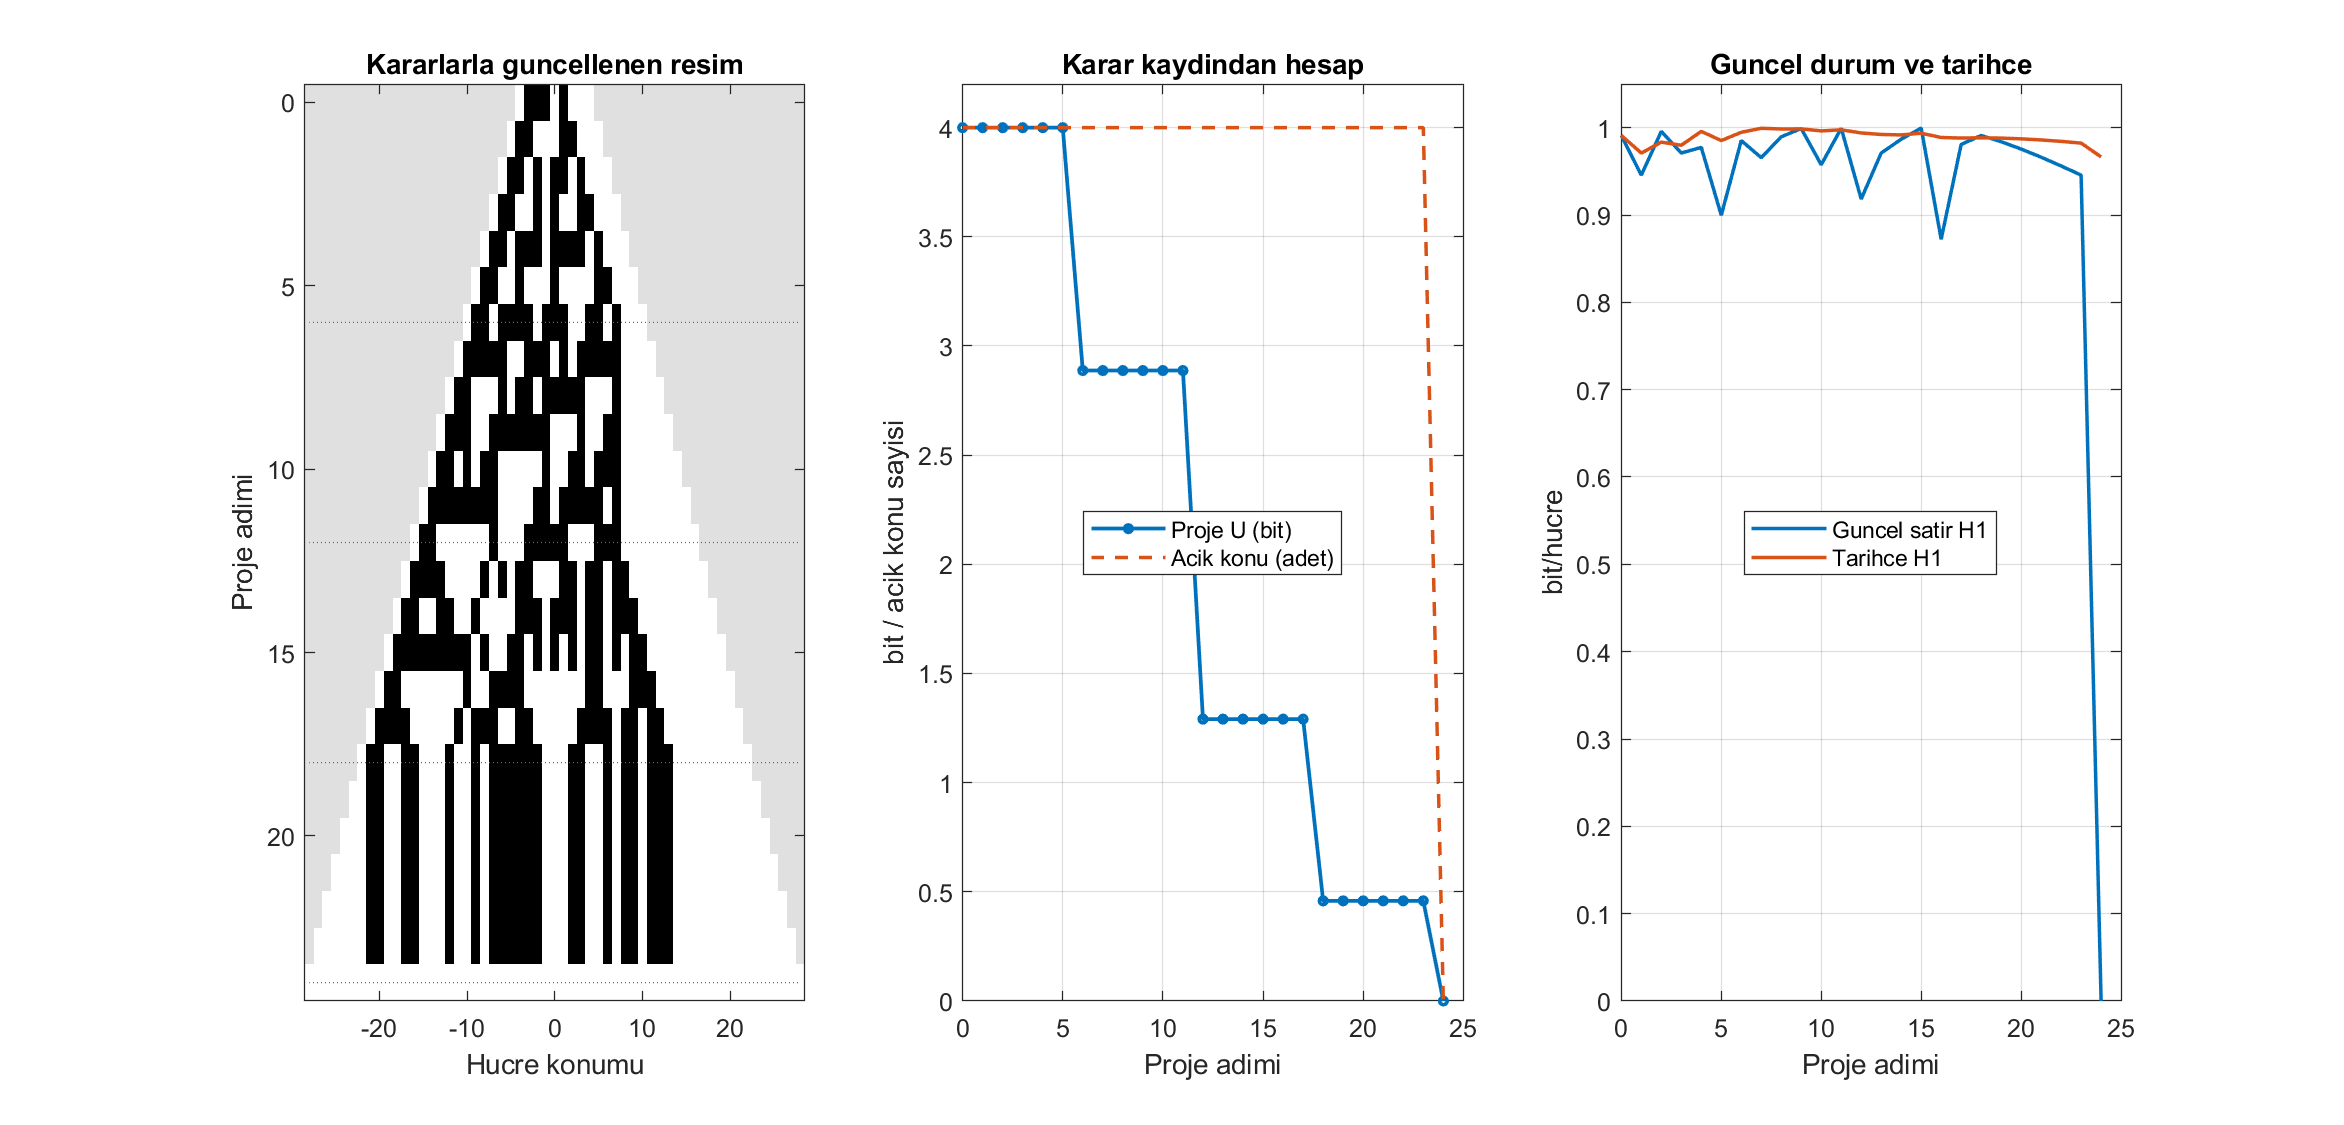
\includegraphics[width=\linewidth]{assets/method_4.png}\end{center}
\begin{center}\small\begin{tabular}{r p{46mm} p{95mm}}\toprule $t$ & Ara çalışma & Karar veya çıktı\\\midrule
6 & İlk karşılaştırmalı ara çalışma & Her konu için hedef seçeneğe 4:1 olabilirlik oranı. \\
12 & İkinci bağımsız ara çalışma & Aynı varsayımsal kanıt oranı ile güncelleme. \\
18 & Üçüncü bağımsız ara çalışma & Güven artar; hiçbir aday olasılığı sıfır değildir. \\
24 & Bağlayıcı tasarım ve kabul kararı & 1011 seçilir, uygulanır ve kabul edilir; kesin kapanış. \\
\bottomrule\end{tabular}\end{center}
\textbf{Yorum.} Olasılıksal kanıt belirsizliği azaltır fakat sonlu ve pozitif olabilirliklerle tam sıfır üretmez. Son adımda ölçümden otomatik kesinlik çıkarılmıyor: proje bir tasarımı bağlayıcı olarak seçip kapsamını kapatıyor. Böylece sıfır olan nicelik, kabul edilmiş ürün tanımı üzerindeki açık karar belirsizliğidir.

\textbf{Sonuç.} Başarılı kabul girdisi altında tek paket 1011 kalır; $U_{24}=0$, $O_{24}=0$, $V_{24}=4$ ve son satır tamamen beyazdır. Geçmiş satırlar korunur.

\page{Yöntem 4/5 | Hesap ve izlenebilirlik}{Kanıt güncellemesi ve kesin kabul: sayısal sonuçlar}
Her konu için başlangıç oranı $1:1$; her bağımsız kanıtın olabilirlik oranı $4:1$ kabul edilir. $k$ kanıttan sonra $q_k=4^k/(1+4^k)$ ve $U=4h_2(q_k)$. $q_1=0{,}8$, $q_2=16/17$, $q_3=64/65$; sonlu $k$ için $U>0$. Son kapı bu yumuşak güncellemeden farklı, bağlayıcı bir seçimdir.
\begin{center}\small\begin{tabular}{rrrrrrr}\toprule $t$ & Aday & Açık konu & Proje $U$ & Satır $H_1$ & Geçmiş $H_1$ & Kabul\\\midrule
0 & 16 & 4 & 4,0000 & 0,9911 & 0,9911 & 0/4 \\
1 & 16 & 4 & 4,0000 & 0,9457 & 0,9710 & 0/4 \\
2 & 16 & 4 & 4,0000 & 0,9957 & 0,9834 & 0/4 \\
3 & 16 & 4 & 4,0000 & 0,9710 & 0,9799 & 0/4 \\
4 & 16 & 4 & 4,0000 & 0,9774 & 0,9957 & 0/4 \\
5 & 16 & 4 & 4,0000 & 0,8997 & 0,9852 & 0/4 \\
6 & 16 & 4 & 2,8877 & 0,9852 & 0,9947 & 0/4 \\
7 & 16 & 4 & 2,8877 & 0,9656 & 0,9993 & 0/4 \\
8 & 16 & 4 & 2,8877 & 0,9896 & 0,9985 & 0/4 \\
9 & 16 & 4 & 2,8877 & 0,9990 & 0,9986 & 0/4 \\
10 & 16 & 4 & 2,8877 & 0,9576 & 0,9963 & 0/4 \\
11 & 16 & 4 & 2,8877 & 0,9992 & 0,9975 & 0/4 \\
12 & 16 & 4 & 1,2910 & 0,9183 & 0,9939 & 0/4 \\
13 & 16 & 4 & 1,2910 & 0,9710 & 0,9922 & 0/4 \\
14 & 16 & 4 & 1,2910 & 0,9868 & 0,9917 & 0/4 \\
15 & 16 & 4 & 1,2910 & 0,9995 & 0,9937 & 0/4 \\
16 & 16 & 4 & 1,2910 & 0,8722 & 0,9888 & 0/4 \\
17 & 16 & 4 & 1,2910 & 0,9808 & 0,9881 & 0/4 \\
18 & 16 & 4 & 0,4587 & 0,9911 & 0,9884 & 0/4 \\
19 & 16 & 4 & 0,4587 & 0,9839 & 0,9880 & 0/4 \\
20 & 16 & 4 & 0,4587 & 0,9755 & 0,9872 & 0/4 \\
21 & 16 & 4 & 0,4587 & 0,9662 & 0,9859 & 0/4 \\
22 & 16 & 4 & 0,4587 & 0,9562 & 0,9843 & 0/4 \\
23 & 16 & 4 & 0,4587 & 0,9457 & 0,9823 & 0/4 \\
24 & 1 & 0 & 0,0000 & 0,0000 & 0,9665 & 4/4 \\
\bottomrule\end{tabular}\end{center}
\textbf{Hesap ayrımı.} Proje $U$ değeri paket olasılıklarından; satır ve geçmiş değerleri hücre frekanslarından hesaplanır. Hepsi bit tabanını kullanır, fakat aynı rastgele değişkenin entropisi değildir. Son satırın genişliği 57, geçmişin alanı 825 hücredir.

\page{Yöntem 5/5 | Proje akışı}{8\quad Prototiplerle aday eleme}
\textbf{Ara çalışma kuralları.} $t=1\!:\!6,\ 7\!:\!12,\ 13\!:\!18,\ 19\!:\!24$ evrelerinde sırasıyla 110, 30, 184, 204 uygulanır. Karar operatörü bu yerel kurallardan ayrıdır.
\begin{center}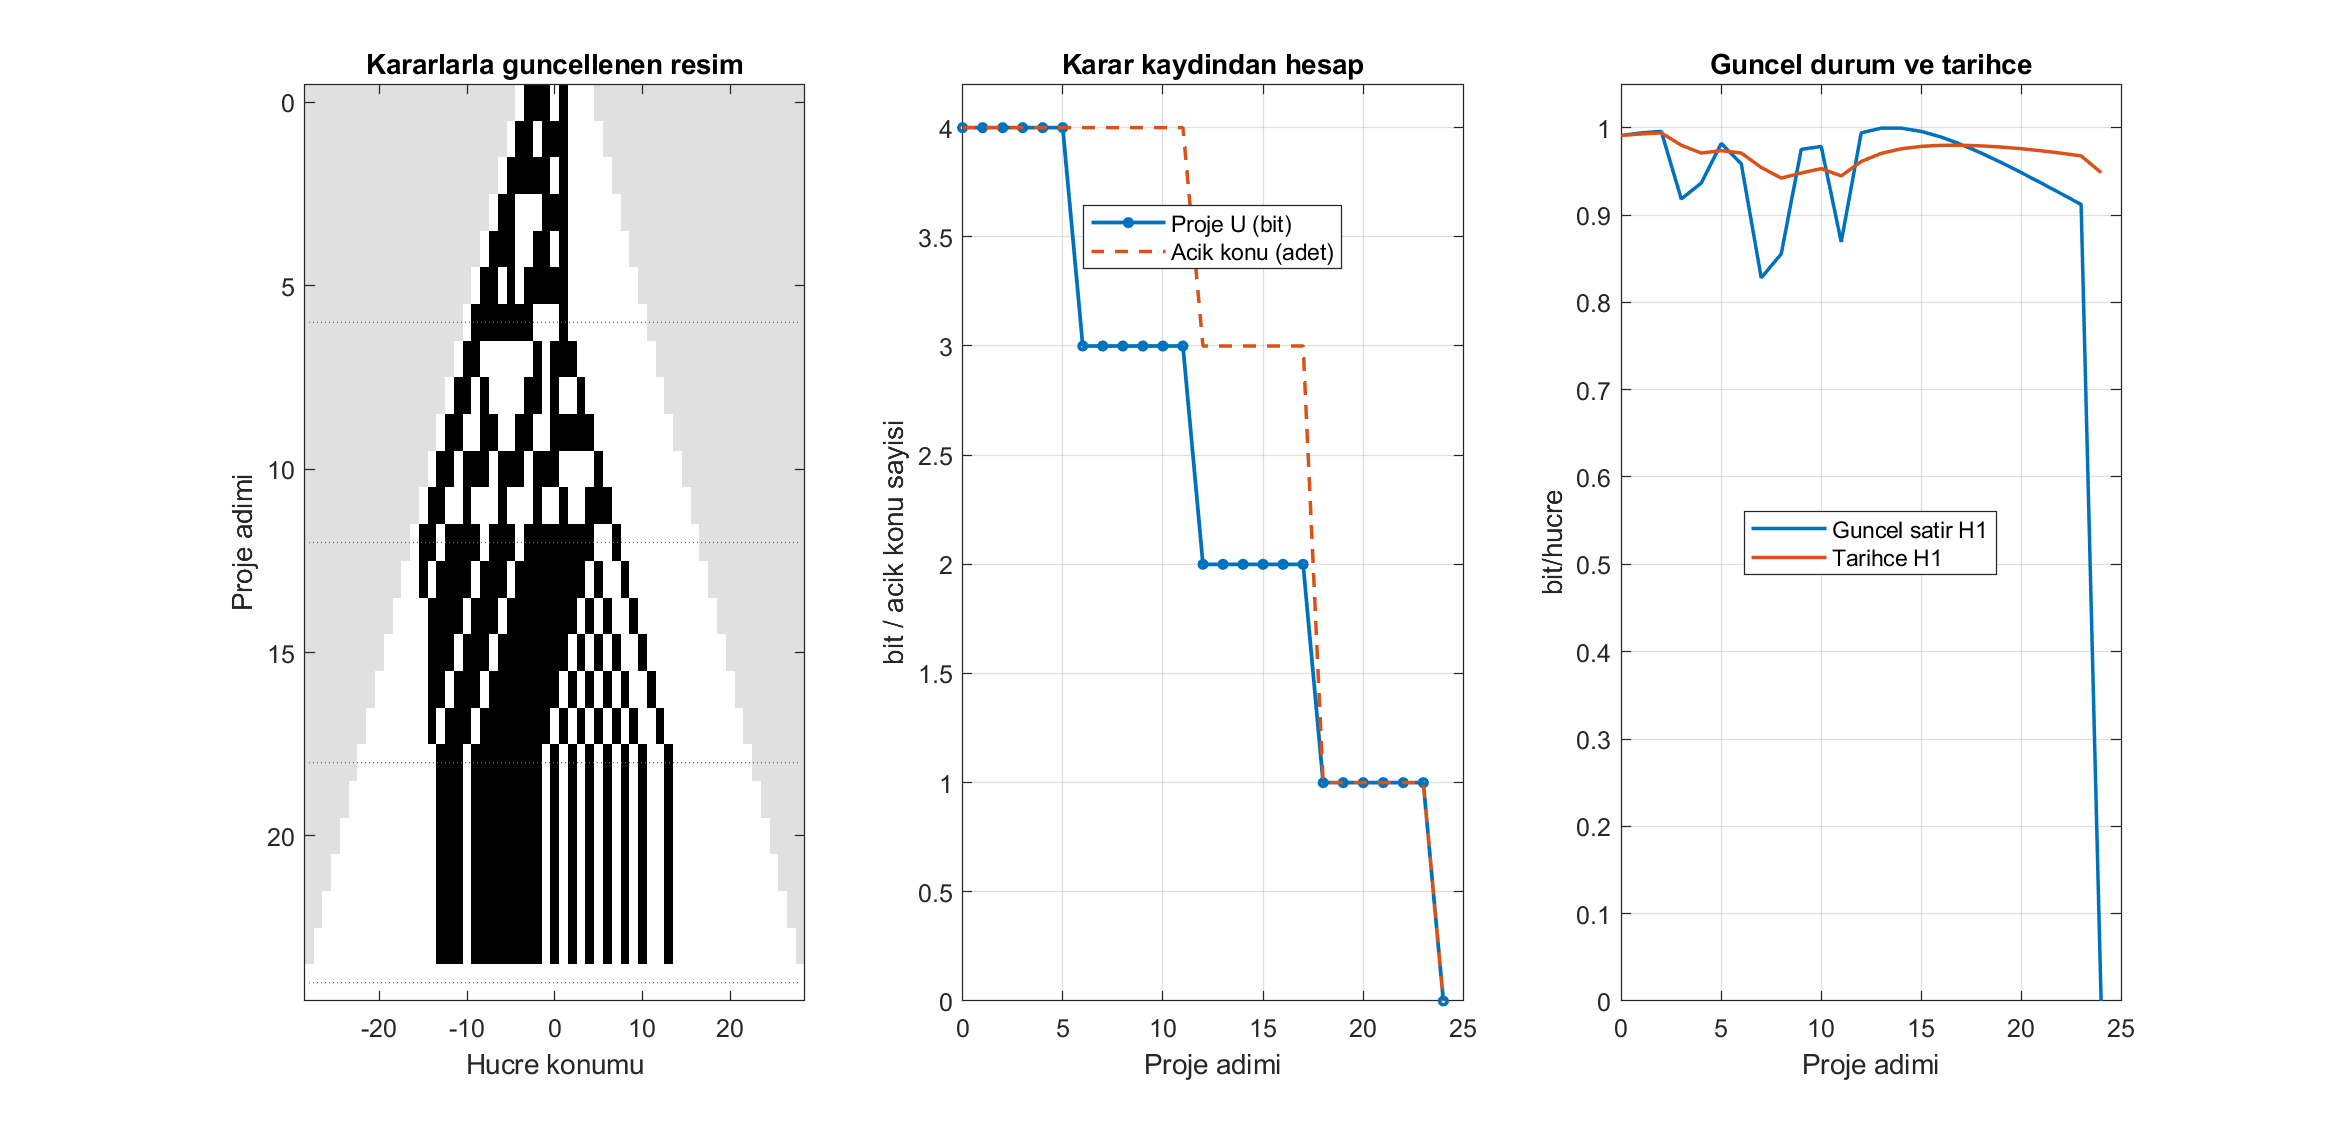
\includegraphics[width=\linewidth]{assets/method_5.png}\end{center}
\begin{center}\small\begin{tabular}{r p{46mm} p{95mm}}\toprule $t$ & Ara çalışma & Karar veya çıktı\\\midrule
6 & Kavram prototiplerinin elemesi & 16 adaydan sıralamadaki ilk 8 kalır. \\
12 & Masaüstü mekanizma deneyi & 8 adaydan ilk 4 kalır. \\
18 & İşlevsel prototip kıyaslaması & 4 adaydan ilk 2 kalır: 1011 ve 1010. \\
24 & Tam çevrim testi ve son seçim & 1011 tek aday kalır; ürün kabulü tamamlanır. \\
\bottomrule\end{tabular}\end{center}
\textbf{Yorum.} Değerlendirme bütün aday paketlerini karşılaştırır; tek tek konuları sabitlemek zorunda değildir. Dolayısıyla aday sayısı azalırken bir süre dört konunun tamamı açık kalabilir. Sıralama bu raporda örnek girdi olarak verilmiştir; gerçek projede her elemenin test veya karar kaydı bulunmalıdır.

\textbf{Sonuç.} Başarılı kabul girdisi altında tek paket 1011 kalır; $U_{24}=0$, $O_{24}=0$, $V_{24}=4$ ve son satır tamamen beyazdır. Geçmiş satırlar korunur.

\page{Yöntem 5/5 | Hesap ve izlenebilirlik}{Prototiplerle aday eleme: sayısal sonuçlar}
Örnek tercih sırası, en iyiden başlayarak aday kimlikleriyle $11,10,3,15,9,7,2,14,1,13,8,6,5,0,12,4$ olarak verilmiştir. Kimlik, dört bitlik ABCD paketinin onluk karşılığıdır. Her kapıda ilk yarı tutulur. Bu sıra ölçülmüş prototip puanı değildir; deney planını göstermek için verilmiş girdidir.
\begin{center}\small\begin{tabular}{rrrrrrr}\toprule $t$ & Aday & Açık konu & Proje $U$ & Satır $H_1$ & Geçmiş $H_1$ & Kabul\\\midrule
0 & 16 & 4 & 4,0000 & 0,9911 & 0,9911 & 0/4 \\
1 & 16 & 4 & 4,0000 & 0,9940 & 0,9928 & 0/4 \\
2 & 16 & 4 & 4,0000 & 0,9957 & 0,9940 & 0/4 \\
3 & 16 & 4 & 4,0000 & 0,9183 & 0,9799 & 0/4 \\
4 & 16 & 4 & 4,0000 & 0,9367 & 0,9710 & 0/4 \\
5 & 16 & 4 & 4,0000 & 0,9819 & 0,9737 & 0/4 \\
6 & 8 & 4 & 3,0000 & 0,9587 & 0,9710 & 0/4 \\
7 & 8 & 4 & 3,0000 & 0,8281 & 0,9544 & 0/4 \\
8 & 8 & 4 & 3,0000 & 0,8555 & 0,9422 & 0/4 \\
9 & 8 & 4 & 3,0000 & 0,9751 & 0,9481 & 0/4 \\
10 & 8 & 4 & 3,0000 & 0,9784 & 0,9531 & 0/4 \\
11 & 8 & 4 & 3,0000 & 0,8691 & 0,9447 & 0/4 \\
12 & 4 & 3 & 2,0000 & 0,9940 & 0,9612 & 0/4 \\
13 & 4 & 3 & 2,0000 & 0,9994 & 0,9706 & 0/4 \\
14 & 4 & 3 & 2,0000 & 0,9995 & 0,9758 & 0/4 \\
15 & 4 & 3 & 2,0000 & 0,9957 & 0,9786 & 0/4 \\
16 & 4 & 3 & 2,0000 & 0,9892 & 0,9798 & 0/4 \\
17 & 4 & 3 & 2,0000 & 0,9808 & 0,9799 & 0/4 \\
18 & 2 & 1 & 1,0000 & 0,9710 & 0,9792 & 0/4 \\
19 & 2 & 1 & 1,0000 & 0,9601 & 0,9778 & 0/4 \\
20 & 2 & 1 & 1,0000 & 0,9486 & 0,9759 & 0/4 \\
21 & 2 & 1 & 1,0000 & 0,9367 & 0,9735 & 0/4 \\
22 & 2 & 1 & 1,0000 & 0,9245 & 0,9708 & 0/4 \\
23 & 2 & 1 & 1,0000 & 0,9121 & 0,9677 & 0/4 \\
24 & 1 & 0 & 0,0000 & 0,0000 & 0,9486 & 4/4 \\
\bottomrule\end{tabular}\end{center}
\textbf{Hesap ayrımı.} Proje $U$ değeri paket olasılıklarından; satır ve geçmiş değerleri hücre frekanslarından hesaplanır. Hepsi bit tabanını kullanır, fakat aynı rastgele değişkenin entropisi değildir. Son satırın genişliği 57, geçmişin alanı 825 hücredir.
\page{Yöntemlerin karşılaştırılması}{9\quad Projeyi ne kapatıyor?}
\begin{center}\small\begin{tabular}{c p{47mm} p{65mm} r}\toprule
Yöntem & Kapanışı üreten işlem & En önemli ayrım & Geçmiş $H_1$\\\midrule
1 & Her kapıda tek konu kararı & İzlenebilir fakat sıralı bağımlılık var. & 0,6996 \\
2 & İki iş paketinin bütünleştirilmesi & Alt sistemlerden sonra ortak kabul gerekir. & 0,7889 \\
3 & Bağlantı kararlarının yayılması & Çelişen kısıtlar boş küme doğurabilir. & 0,4435 \\
4 & Olasılık güncellemesi + kesin seçim & Pozitif kanıt tek başına tam sıfır yapmaz. & 0,9665 \\
5 & Aday paketlerin aşamalı elenmesi & Az aday, az açık konu demek değildir. & 0,9486 \\
\bottomrule\end{tabular}\end{center}
Beş yöntemde de son durum aynıdır: $U=0$, açık konu sayısı 0, doğrulanmış
kayıt sayısı 4 ve güncel resim entropisi 0. Geçmiş resim entropileri farklıdır;
bu değerleri yöntem başarısı veya maliyeti sıralaması olarak kullanmıyoruz.
Kural dizileri ve karar takvimleri değiştiği için geçmiş izler farklılaşır.

\section*{Proje için önerilen kullanım}
İlk uygulamada sıralı karar kapıları yöntemi, açık konu ile karar arasındaki
bağı net gösterir. İkinci deneyde aynı karar kayıtları paralel akışta yürütülerek
iş paketi etkileşimleri incelenebilir. Kanıt güncellemesi yöntemi ise
``yüksek güven'' ile ``kapsamı bağlayıcı olarak kapatma'' ayrımını gösterir.

\textbf{Araştırma sorusu.} Aynı nihai tasarıma ulaşan projeler, karar sırası,
aday sayısı, yeniden açılan konu sayısı ve iş yükü bakımından nasıl farklılaşır?
Bu raporun grafikleri böyle bir deneyin görsel altyapısını verir.

\textbf{Sonraki gerçek deneyin kayıtları.} Her karar için kimlik, ilgili konu,
önceki adaylar, yeni adaylar, kullanılan çalışma/test çıktısı, karar veren kişi,
tarih ve yeniden açılma koşulu tutulmalıdır. Prototip başarısızlıkları da
kaydedilmelidir. Yalnız başarı yollarını gösteren bu simülasyon, yöntemlerin
gerçek dünyadaki başarı oranını karşılaştırmaz.

\textbf{Wolfram ile ilişki.} Yerel kuralların karmaşık görünen izler üretmesi
ve gözlemcinin kullandığı betimlemenin önemi, Wolfram'ın tartışmasından
esinlenir [1]. Burada eklenen karar kaydı ve kapanış operatörü ise bu proje
için kurulmuş ayrı bir mühendislik modelidir. Termodinamiğin ikinci yasasından
proje belirsizliğinin sıfıra ineceği sonucu türetilmemektedir.

\page{Kaynaklar ve yeniden üretim}{10\quad MATLAB, TeX ve doğrulama}
Kaynak paketini bir klasöre açıp MATLAB içinde şu komutu çalıştırın:
\begin{verbatim}
build_project_methods(fullfile(pwd,'assets'))
\end{verbatim}
MATLAB R2018b ile çalıştırılmıştır; ek toolbox gerekmez. Her yöntem için
grafik (PNG ve FIG), 25 satırlık hesap tablosu ve 16 adayın olasılık tablosu üretilir.
\begin{center}\small\begin{tabular}{p{64mm}p{85mm}}\toprule
Dosya & İçerik\\\midrule
\texttt{build\_project\_methods.m} & Beş akış, konu etiketleri, karar operatörü, grafikler\\
\texttt{pattern\_entropy.m} & Tekli ve ikili desen frekans entropisi\\
\texttt{assets/method\_N.csv} & Adım, kural, bit dizisi, konu sayısı, entropiler, kabul sayısı\\
\texttt{assets/posterior\_N.csv} & Her adımda 0000--1111 paketlerinin olasılıkları\\
\texttt{proje\_bes\_yontem.tex} & Düzenlenebilir rapor kaynağı\\\bottomrule
\end{tabular}\end{center}
\textbf{Bağımsız kontrol.} Beş yöntemin toplam 125 satırı Python ile ayrıca
üretilmiştir. Bit dizileri, etiket süzme sonucu, aday ve açık konu sayıları,
geçici resimden çıkarılan hücre sayıları ve bütün entropiler MATLAB çıktısıyla
$10^{-12}$ mutlak tolerans içinde eşleşmiştir. 2000 aday olasılığı da kontrol
edilmiştir. Son durum koşulları ayrıca doğrulanmıştır.

\textbf{Model sınırı.} Kabul sütunundaki 4/4, başarılı senaryo girdisidir;
yazılım fiziksel test yapmaz. Kuralları değiştirerek farklı resimler elde
edilebilir. Proje entropisini kural numarası değil, aday/karar kaydı belirler.
Yeni konu eklenmesi ve başarısız testle geri dönüş bu sürümün çalışan dalında
modellenmemiştir; gerçek proje uygulamasında eklenmelidir.

TeX derlemesi (aynı komut iki kez):
\begin{verbatim}
xelatex -interaction=nonstopmode -halt-on-error
    proje_bes_yontem.tex
\end{verbatim}
Komut tek satırda yazılır. Cambria, Calibri ve Consolas yazı tipleri kullanılır.

\textbf{Kaynak [1].} S. Wolfram (2023), \emph{Computational Foundations for
the Second Law of Thermodynamics}. Stephen Wolfram Writings, 3 Şubat 2023.
\par\small\texttt{https://writings.stephenwolfram.com/2023/02/}\par
\texttt{computational-foundations-for-the-second-law-of-thermodynamics/}
\end{document}
